% Draw rotation group properties
\documentclass[crop,tikz]{standalone}
\usepackage{pgfplots}
\usepackage{tikz-3dplot}
\begin{document}

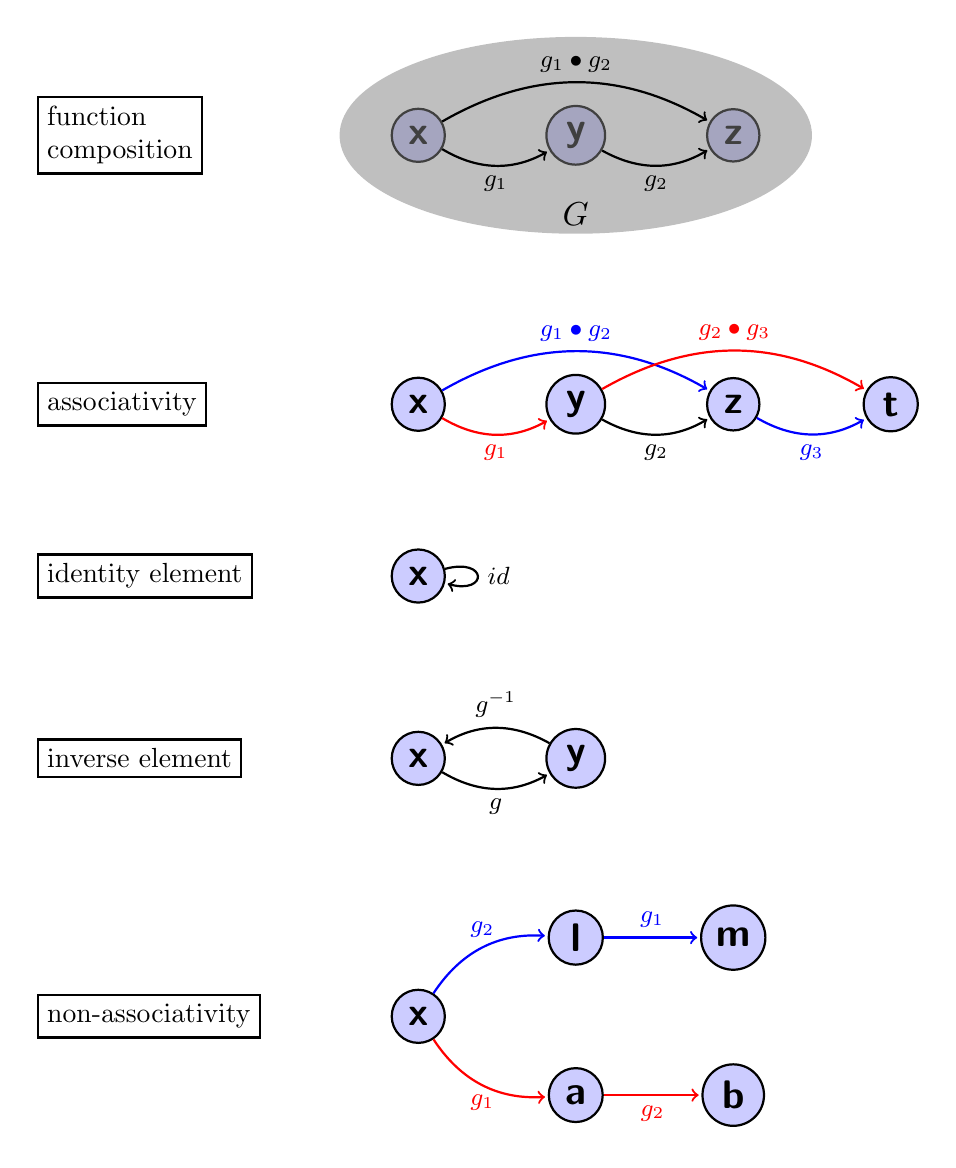
\begin{tikzpicture}[->,shorten >=1pt,auto,node distance=2cm,
  thick,main node/.style={circle,fill=blue!20,draw,font=\sffamily\Large\bfseries}]

\matrix[column sep = 1cm, row sep = 1cm]{
  \node [draw, anchor=west, align=left] {function \\ composition};
&
  \node[main node] (1) {x};
  \node[main node] (2) [right of=1] {y};
  \node[main node] (3) [right of=2] {z};
  \path [draw=none,fill=gray,semitransparent] (2,0) ellipse (3cm and 1.25cm);
  \node [scale=1.2] at (2,-1) {$G$};
  \path[every node/.style={font=\sffamily\small}]
    (1) edge [bend right] node [below] {$g_{1}$} (2)
        edge [bend left]  node {$g_{1} \bullet g_{2}$} (3)
    (2) edge [bend right] node [below] {$g_{2}$} (3);
\\
  \node [draw, anchor=west, align=left] {associativity};
&
  \node[main node] (1) {x};
  \node[main node] (2) [right of=1] {y};
  \node[main node] (3) [right of=2] {z};
  \node[main node] (4) [right of=3] {t};

  \path[every node/.style={font=\sffamily\small}]
    (1) edge [bend right,red] node [below] {$g_{1}$} (2)
        edge [bend left,blue]  node {$g_{1} \bullet g_{2}$} (3)
    (2) edge [bend right] node [below] {$g_{2}$} (3)
        edge [bend left,red]  node {$g_{2} \bullet g_{3}$} (4)
    (3) edge [bend right,blue] node [below] {$g_{3}$} (4);
\\
  \node [draw, anchor=west, align=left] {identity element};
&
  \node[main node] (1) {x};

  \path[every node/.style={font=\sffamily\small}]
    (1) edge [loop right] node [right] {$id$} (1);
\\
  \node [draw, anchor=west, align=left] {inverse element};
&
  \node[main node] (1) {x};
  \node[main node] (2) [right of=1] {y};

  \path[every node/.style={font=\sffamily\small}]
    (1) edge [bend right] node [below] {$g$} (2)
    (2) edge [bend right] node [above] {$g^{-1}$} (1);
\\
  \node [draw, anchor=west, align=left] {non-associativity};
&
  \node[main node] (1) at (0,0){x};
  \node[main node] (2) at (2,-1) {a};
  \node[main node] (3) at (4,-1) {b};
  \node[main node] (4) at (2,1) {l};
  \node[main node] (5) at (4,1) {m};

  \path[every node/.style={font=\sffamily\small}]
    (1) edge [bend right,red] node [below] {$g_{1}$} (2)
        edge [bend left,blue] node [above] {$g_{2}$} (4)
    (2) edge [red] node [below] {$g_{2}$} (3)
    (4) edge [blue] node [above] {$g_{1}$} (5);
\\
};
\end{tikzpicture}

\end{document}